\documentclass[10pt]{article}
\usepackage[margin=0.82in]{geometry}
\usepackage{booktabs,tabularx,array,amsmath,hyperref,xcolor,graphicx,enumitem}
\usepackage{tikz}
\usetikzlibrary{arrows.meta,positioning,calc}
\definecolor{ink}{HTML}{101820}
\definecolor{teal}{HTML}{007C78}
\definecolor{amber}{HTML}{C97900}
\definecolor{coral}{HTML}{C34545}
\definecolor{violet}{HTML}{7552A8}
\hypersetup{colorlinks=true,urlcolor=teal,linkcolor=teal,pdftitle={Building a Miniature AI Factory},pdfauthor={Tanvir Ahmed},pdfsubject={Post-training, inference engines, and provider systems}}
\setlength{\parskip}{2.5pt}
\title{Building a Miniature AI Factory:\\ \large Post-Training, Inference Engines, and Provider Systems}
\author{Tanvir Ahmed\\\small \url{https://github.com/mailtotanvir/Nano-RL-Inference}}
\date{September 2026}
\begin{document}\sloppy\maketitle

\begin{abstract}
Modern AI systems are often described as a model plus an API. That shorthand hides the engineering that determines whether a training result can become a reliable product: frozen data boundaries, reward contracts, reference policies, rollout collection, inference engines, model routing, authentication, rate limits, usage accounting, and artifact custody. This paper documents a constrained, end-to-end replication of that chain using Qwen/Qwen2.5-0.5B-Instruct, a deterministic arithmetic environment, LoRA supervised fine-tuning (SFT), and four reinforcement-learning families: REINFORCE, PPO, RLOO, and GRPO. The study selected a 0.5B model and a single NVIDIA L4 specifically to make the full loop affordable, inspectable, and disposable rather than to claim frontier capability. Training used 512 addition/subtraction examples; evaluation withheld an entire division-template family of 128 examples. A three-seed, 21-cell campaign found the same held-out result, 4/128, for every saved adapter. This is not evidence that the methods are equivalent. It is evidence that reward-bearing optimization did not transfer under this strict contract. We also run the merged adapter through vLLM and SGLang, and expose local and live backends through an OpenAI-compatible FastAPI provider with routing, authentication, rate limits, streaming, metrics, and usage accounting. The contribution is an explainer backed by executable artifacts: what each RL family is buying, where serving changes the problem, why a favorable internal reward is not a generalization claim, and how to retain evidence after a short-lived GPU has been deleted.
\end{abstract}

\section{Introduction}
Modern AI systems are often described as a model plus an API. That shorthand is useful until it hides the engineering that determines whether a training result can become a reliable product: frozen data boundaries, reward contracts, reference policies, rollout collection, inference engines, model routing, authentication, rate limits, usage accounting, and artifact custody.

This paper documents a constrained, end-to-end reconstruction of that chain. It is not a claim that a 0.5B model is competitive with frontier reasoning systems, nor a claim that five RL families are interchangeable. It is a practical explainer: we build small but real versions of the post-training and serving components, then retain enough evidence to distinguish an internal optimization signal from transferable behavior and a functioning engine from a usable provider.

The organizing question is therefore practical: \emph{what does it take to build, inspect, and operate a miniature version of the post-training and inference stack used by modern AI products?} The remainder follows the construction order. Section~\ref{sec:design} establishes the experimental and architectural choices. Section~\ref{sec:evidence} explains why evidence custody is part of the system. The subsequent sections unpack the learning loops, results, serving tradeoffs, provider ecosystem, and lessons.

\begin{center}
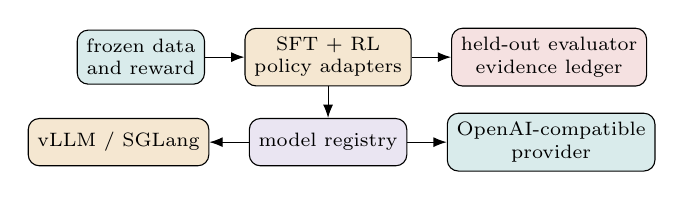
\begin{tikzpicture}[node distance=4mm and 5mm,every node/.style={draw,rounded corners,align=center,minimum height=6mm,font=\scriptsize},>=Latex]
\node[fill=teal!15] (data) {frozen data\\and reward};
\node[fill=amber!18,right=of data] (train) {SFT + RL\\policy adapters};
\node[fill=coral!16,right=of train] (eval) {held-out evaluator\\evidence ledger};
\node[fill=violet!15,below=of train] (registry) {model registry};
\node[fill=amber!18,left=of registry] (engines) {vLLM / SGLang};
\node[fill=teal!15,right=of registry] (provider) {OpenAI-compatible\\provider};
\draw[->] (data)--(train); \draw[->] (train)--(eval); \draw[->](train)--(registry); \draw[->](registry)--(engines); \draw[->](registry)--(provider);
\end{tikzpicture}
\end{center}

\section{Experiment design and architectural choices}\label{sec:design}
\subsection{One small model, one L4, and LoRA adapters}
The base is \texttt{Qwen/Qwen2.5-0.5B-Instruct}. A 0.5B instruct model is large enough to exercise realistic tokenization, chat templates, adapter loading, generation, reference-policy comparisons, and server integration, while remaining feasible on one L4. The purpose is iteration economics: if the entire train, evaluate, serve, collect, checksum, and teardown loop cannot be completed under a small budget, it is difficult to inspect its failure modes honestly.

SFT uses PEFT LoRA with rank 8, alpha 16, 0.05 dropout, and targets \texttt{q\_proj} and \texttt{v\_proj}. One epoch, per-device batch size four, gradient accumulation four, and learning rate $2\times10^{-4}$ form the cold-start policy. These are not claimed as optimal settings. They were chosen to create a stable, reproducible adapter that each RL method could inherit, rather than letting every method begin by rediscovering answer format.

\subsection{A task where correctness is cheap, but transfer is not}
The environment has 512 generated train examples from addition and subtraction templates. The held-out set contains 128 division-template examples. The reward uses conservative normalization and exact numeric matching. That makes the reward auditable: a response is either the expected integer or reduced fraction, or it is not. It also creates a harsh distinction between fitting a prompt family and transferring across one.

This choice is important. A high-quality learned reward model could obscure whether a policy was rewarded because of its behavior or because of a judge's preference. Here, the reward is not the hard part. The hard part is whether a policy optimized on one family carries useful structure into another family.

\begin{table*}[t]
\centering\small
\caption{Method selection is a tradeoff among feedback shape, variance, stability, and operational cost. These are the implemented miniature forms, not a claim of exhaustive or production-scale implementations.}
\begin{tabularx}{\textwidth}{p{.14\textwidth} p{.22\textwidth} p{.27\textwidth} X}
\toprule
Method & What it changes & Why build it here & Main tradeoff to watch \\
\midrule
SFT & Fits verified answer demonstrations & Establishes a common policy and formatting prior & Cannot improve beyond the coverage of demonstrations \\
REINFORCE & Raises probability of rewarded sampled actions & Simplest direct reward-to-gradient baseline & Sparse reward makes the estimate high variance \\
PPO & Clips policy-ratio movement and adds KL pressure & Shows how a useful policy can be protected from destructive updates & Requires old-policy bookkeeping, advantages, and a reference policy \\
RLOO & Uses sibling rollouts as a leave-one-out baseline & Reduces variance without fitting a separate learned critic & Needs grouped samples and careful episode construction \\
GRPO & Normalizes reward within a response group & Replaces a large critic with relative group evidence for verifiable tasks & Rollout count, group composition, KL, and generation cost become first-order settings \\
\bottomrule
\end{tabularx}
\end{table*}

\section{Evidence discipline and campaign custody}\label{sec:evidence}
The project treats evidence as a system boundary, not a publication task postponed until the end. Every training cell receives an explicit seed, output directory, SFT-adapter dependency, and metric path. A successful adapter is evaluated immediately after training, so the record binds the training invocation to the model artifact and its held-out score rather than leaving evaluation as a later manual step.

The three seeds, 13, 42, and 97, crossed seven method labels, producing 21 lifecycle cells and 21 saved-adapter evaluation files. The campaign ledger records planned, completed, and failed transitions; the final metric-complete campaign recorded 21 completed cells. This discipline also preserves negative evidence. A result that does not improve is not discarded because it does not make a favorable chart.

GPU work used a short-lived on-demand \texttt{g2-standard-8} with one NVIDIA L4 in GCP. The rate captured before campaign work was \$0.853624312 per hour. Artifacts were copied to the laptop and an existing OCI mirror, and their SHA-256 values matched before the VM was deleted. The metric-complete archive hash is maintained in the repository evidence ledger. No idle GPU VM was retained.

The split itself is another evidence control. Training uses 512 generated addition and subtraction examples, while held-out scoring uses 128 division-template examples. Exact-match normalization is conservative. This does not make the evaluation universal, but it prevents a training-family prompt form from silently becoming the definition of success.

\section{Five learning loops, not one algorithm}
\subsection{SFT: the cold start that gives RL a language}
SFT is the control condition and the practical starting point. It teaches the model the chat-format contract and the terse-answer behavior expected by the evaluator. In a product setting, SFT is often the cheapest route when trusted traces already exist. Its limitation is equally important: it can fit the demonstrated surface without acquiring the capability that a withheld task family demands.

\subsection{REINFORCE: the direct but noisy path}
For REINFORCE, a completion is sampled at temperature 0.8 with a 16-token cap. Exact-match reward multiplies the completion log probability:
\[
\mathcal{L}_{\mathrm{REINFORCE}}=-r(y)\frac{1}{|y|}\sum_t\log\pi_\theta(y_t\mid x,y_{<t}).
\]
The attraction is transparency. A reward-bearing answer directly receives more probability mass. The cost is variance: if correct answers are rare, most samples contribute no learning signal. This implementation is therefore an educational baseline for inspecting the reward-to-policy connection, not a claim that naïve REINFORCE is the preferred production post-training method.

\subsection{PPO: conservative movement has its own machinery}
PPO begins at the SFT adapter and keeps a frozen copy as a reference. It computes a sampled-completion probability ratio, clips it to $[0.8,1.2]$, and adds KL pressure with coefficient 0.05:
\[
\begin{aligned}
\mathcal{L}_{\mathrm{PPO}}={}&-\min\left(r_t A_t,\mathrm{clip}(r_t,0.8,1.2)A_t\right)\\
&+0.05\,\mathrm{KL}(\pi_\theta\Vert\pi_{\mathrm{ref}}).
\end{aligned}
\]
The practical reason to build it is not the equation itself. It is to learn what changes when a policy is good enough to damage. PPO buys a trust region-like update boundary, but demands old-policy state, reference behavior, advantages, and careful rollout accounting. The small implementation uses reward as the advantage signal; it intentionally does not claim the full robustness of a production PPO stack.

\subsection{RLOO: a critic replacement with a sampling contract}
RLOO uses four responses per prompt. Each response is judged against the other three, so its advantage is relative to sibling outcomes rather than a learned value function. The pinned TRL 0.15 configuration uses 128 total episodes, four samples per prompt, response length 16, one PPO epoch, learning rate $10^{-5}$, and KL coefficient 0.05. This is useful where adding a critic is undesirable, but it makes batch grouping part of algorithm correctness. A wrong global batch or missing sibling sample is not a harmless implementation detail.

\subsection{GRPO: the group becomes the baseline}
GRPO also uses four generations per prompt, but normalizes reward inside the group. The implementation uses one epoch, batch size four, gradient accumulation four, 16-token completions, and learning rate $10^{-5}$. The appeal is clear for verifiable tasks: a group can provide relative evidence without a large learned critic. The operational lesson is equally clear: generation count, response length, reference behavior, batch divisibility, and KL drift are part of the actual algorithm budget, not afterthoughts.

\subsection{KL estimators: a configuration label is not an ablation}
On 32 development prompts, the SFT policy was compared to the frozen base at the next-token distribution. Mean k1 was 0.06868447 and mean k3 was 0.06909129. These estimates are close here, but k1 is a forward-KL expectation while k3 is a non-negative control-variate form. The campaign includes GRPO k1 and k3 labels for operationally matched execution. The current trainer does not alter its loss formula by that label, so they cannot support a causal estimator claim. This is a general lesson: naming a setting is not the same as measuring its intervention.

\section{Results: why reward did not become transfer}
The campaign completed all 21 cells. Every saved adapter scored 4/128 on every seed in the template-disjoint evaluation (Table \ref{tab:rl-results}). One GRPO cell reported mean rollout reward 0.79167 and KL 0.37643, then scored 4/128 held out. This does not mean reward was wrong. It means the reward answered a narrower question: whether a sampled response matched training-family answers. The held-out set asked whether that learning crossed a template boundary.

\begin{table}[t]\centering\small
\caption{Held-out division-template exact matches. Every cell is 4/128; mean accuracy is 0.03125.}\label{tab:rl-results}
\begin{tabular}{lrrrr}\toprule
Method & S13 & S42 & S97 & Mean \\ \midrule
SFT & 4/128 & 4/128 & 4/128 & .03125 \\
REINFORCE & 4/128 & 4/128 & 4/128 & .03125 \\
PPO & 4/128 & 4/128 & 4/128 & .03125 \\
RLOO & 4/128 & 4/128 & 4/128 & .03125 \\
GRPO & 4/128 & 4/128 & 4/128 & .03125 \\
GRPO k1 label & 4/128 & 4/128 & 4/128 & .03125 \\
GRPO k3 label & 4/128 & 4/128 & 4/128 & .03125 \\ \bottomrule
\end{tabular}\end{table}

The most defensible interpretation is narrow. With this small model, data family, reward, output budget, and training exposure, the listed update rules did not change template-disjoint behavior. It does \emph{not} establish that the methods are generally equivalent, that arithmetic reasoning is impossible for the model, or that more data, a different curriculum, a process reward, or a different evaluation would fail. The result is useful precisely because it prevents an attractive but unsupported story: a rising rollout reward cannot be substituted for generalization.

\section{From adapter to inference service}
A model artifact is not an inference product. The SFT adapter was merged for engine compatibility, then served through vLLM 0.8.3 and SGLang 0.4.4.post1 on the same L4. Both engines were exercised through short, medium, and long request shapes with single-request and concurrency-four cells. Ten requests were measured per cell after warmup. This is a workload probe, not a universal benchmark.

\begin{figure*}[t]\centering
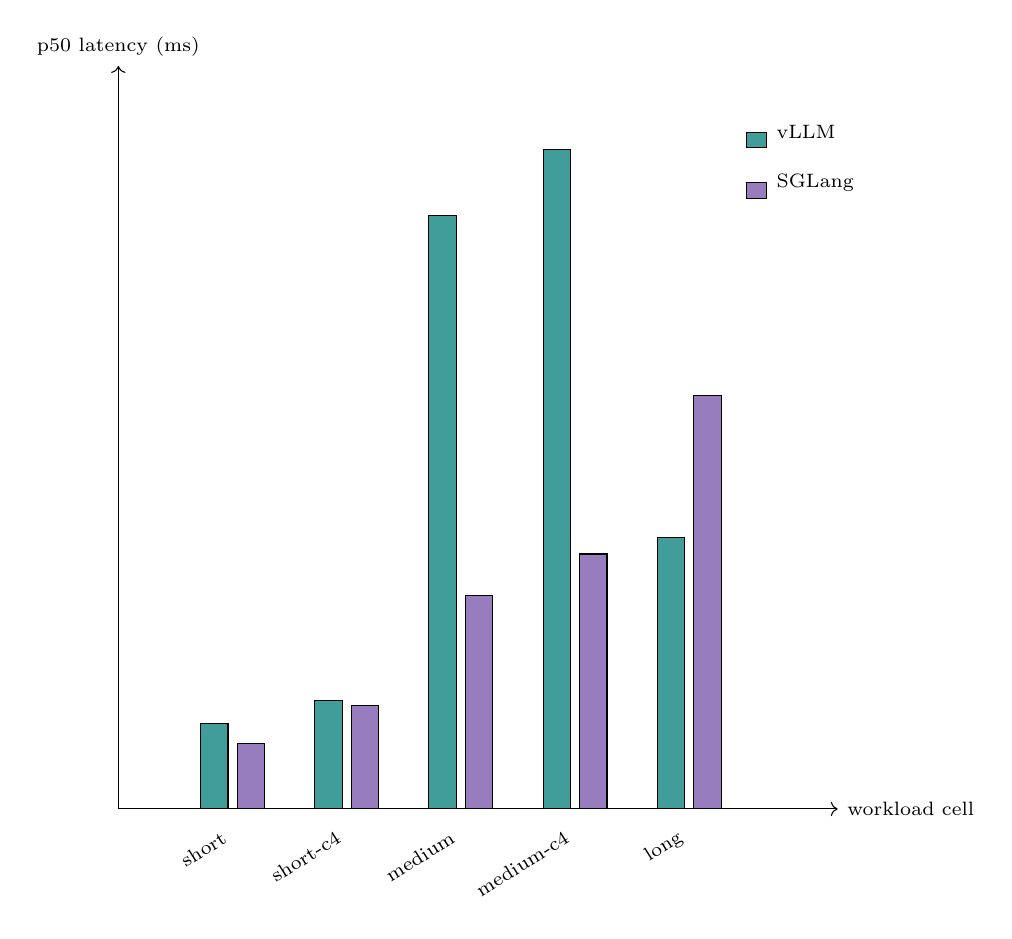
\begin{tikzpicture}[x=1.45cm,y=.008cm,font=\scriptsize]
\draw[->] (0,0)--(6.3,0) node[right]{workload cell};
\draw[->] (0,0)--(0,1180) node[above]{p50 latency (ms)};
\foreach \x/\name/\vllm/\sg in {1/short/136/104,2/short-c4/172/164,3/medium/942/339,4/medium-c4/1048/405,5/long/431/656}{
\draw[fill=teal!75] (\x-.28,0) rectangle (\x-.04,\vllm);
\draw[fill=violet!75] (\x+.04,0) rectangle (\x+.28,\sg);
\node[below,rotate=32,anchor=east] at (\x,-35) {\name};}
\draw[fill=teal!75] (5.5,1050) rectangle +(0.18,25) node[right,black]{vLLM};
\draw[fill=violet!75] (5.5,970) rectangle +(0.18,25) node[right,black]{SGLang};
\end{tikzpicture}
\caption{Measured p50 latency across five workload cells. Lower bars are faster; this view intentionally does not collapse latency and output throughput into one winner.}\label{fig:latency}
\end{figure*}

\begin{table*}[t]\centering\small
\caption{Inference tradeoffs on the same merged adapter and one L4. SGLang led several single-request and medium cells; vLLM retained a higher short concurrency-four aggregate token rate. Output lengths and scheduler behavior differ, so no universal engine ranking follows.}
\resizebox{\textwidth}{!}{\begin{tabular}{lrrrrrr}
\toprule
Workload & vLLM p50 ms & SGLang p50 ms & Faster p50 & vLLM tok/s & SGLang tok/s & Throughput reading \\ \midrule
Short, single & 136.48 & 104.27 & SGLang & 64.90 & 152.04 & SGLang in this cell \\
Short, concurrency 4 & 171.75 & 163.92 & SGLang & 53.59 & 37.63 & vLLM aggregate tok/s \\
Medium, single & 941.76 & 338.78 & SGLang & 67.70 & 188.16 & SGLang in this cell \\
Medium, concurrency 4 & 1047.66 & 405.20 & SGLang & 61.16 & 160.77 & SGLang in this cell \\
Long, single & 430.87 & 656.49 & vLLM & 67.26 & 194.84 & output length matters \\
\bottomrule
\end{tabular}}
\end{table*}

Figure \ref{fig:latency} and the table answer a more useful question than ``which engine wins?'' A serving choice depends on request length, concurrency, queueing, stopping behavior, cache policy, and whether the business requirement values first-token latency, total latency, or aggregate throughput. The long cell makes the point: lower latency and higher reported token throughput can point in different directions when completion behavior differs. A benchmark is a protocol, not a decorative number.

\section{The provider boundary is where engines become an ecosystem}
The FastAPI provider exposes \texttt{/health}, \texttt{/v1/models}, \texttt{/v1/completions}, \texttt{/v1/chat/completions}, \texttt{/v1/responses}, \texttt{/usage}, and \texttt{/metrics}. It validates bearer tokens by hash, resolves a public model identifier through deterministic routing, uses a per-identity token bucket, supports streaming completion events, accounts for requests and token estimates, and exports request metrics.

The design deliberately keeps vLLM, SGLang, and generic remote OpenAI-compatible inference behind a common backend protocol. A client should depend on a stable OpenAI-shaped contract, not on a local server's port, a vendor's model naming convention, or an engine-specific streaming behavior. A live remote-backend acceptance artifact returned \texttt{42}, counted 10 prompt and 1 completion token, and recorded 1578.84 ms latency. This is evidence of a real provider path, not a claim of a public, production-hardened deployment.

\section{Lessons and limitations}
For ML engineers, the transferable pattern is to choose the learning loop from the feedback available. Verified answers invite SFT and group-relative rollouts; expensive or ambiguous rewards demand stronger variance and evaluation controls. For platform teams, the transferable pattern is to place model identity, authentication, routing, quotas, usage, and observability outside the serving engine. For leaders, the cost lesson is that an L4 bill is only affordable learning when the campaign starts ready, produces evidence, and is torn down without losing the result.

The limitations are material. This is one model family, small deterministic data, a strict family-disjoint test, compact educational REINFORCE and PPO implementations, brief engine samples, and no integrated public GCP provider deployment. GRPO k1 and k3 labels are not a loss-formula ablation. This work should be read as a reproducible engineering explainer and evidence record, not a certification, a broad algorithmic comparison, or a leaderboard claim.

\section{Conclusion}
The central result is not that five RL paths were tried or that two engines returned latency numbers. It is that a miniature AI factory made their dependencies inspectable. Training can improve a local reward while failing to transfer. A model can serve through two engines without either engine being universally superior. An API can look compatible while still needing governance around identity, cost, and evidence. Building the complete chain made those distinctions concrete. The model is one component; the accountable system around it is the artifact.

\paragraph{Reproducibility.} Code, frozen data manifest, campaign ledger, per-seed metrics, benchmark JSON, and claim-evidence matrix are in \url{https://github.com/mailtotanvir/Nano-RL-Inference}. The publication evidence is not yet a public Zenodo record or Hugging Face release.
\end{document}
